\documentclass[10pt]{iopart}
% \usepackage{setstack}
\usepackage{iopams}

\usepackage{physics}

\usepackage{todonotes}
\usepackage{cite}
\usepackage{lipsum}
\usepackage{hyperref}
\usepackage{csquotes}

\newcommand{\PHYSICS}{\textbf{PHYSICS!!!!}
}
\newcommand{\R}{\mathbb{R}}
%\newcommand{\ddd}{\mathrm{d}}
\newcommand{\rdd}{~\mathrm{d}}
\newcommand{\p}{\partial}
\newcommand{\st}{\mathrm{~s.t.~}}
\newcommand{\set}[1]{\left\{#1\right\}}

\def\SI{Slimpletic Integrator}
\def\SymI{{Sympletic integrator}}
\newcommand{\autodiff}{automatic-differentiation}
\def\vbq{\vb{q}}
\newcommand{\orgimpl}{\textit{original implementation}}
\newcommand{\updimpl}{\textit{updated implementation}}

\begin{document}
\ioptwocol[{
\title{Iterations on the slimpletic integrator and its applications to physically informed loss functions}
\author{J D Coles$^1$}
\address{$^1$ Department of Physics, University of Bath, Claverton Down, Bath BA2 7AY, UK}
\begin{abstract}
\lipsum[1]
\end{abstract}
}]

\section{Introduction}

Neural networks (NNs) and other machine learning (ML) techniques are becoming an increasingly important tool in of modern research process. This is due to their wide application in data-intensive problems, and ability to make progress where prior computational methods have proved otherwise intractable.

The primary method of training ML models involves the construction of a loss function or equivalently reward function. This frames the training process as a high-dimensionality optimisation problem. In this setting, the various parameters of the model are varied such as to minimise the aggregate loss of the model's action over a large collection of inputs when compared to known corresponding outputs. It is thus the loss function that grounds the model in a given problem. Their construction varies but they exhibit some general characteristics as will be discussed.

% Cite: https://en.wikipedia.org/wiki/Symplectic_integrator and DT's unpublished paper.
\todo{check with DT about the wording of "canonical symplectic 2-form of the system"}
\SymI{}s are numerical integrators for Hamiltonian systems which preserve the canonical symplectic 2-form of the system. 
This makes them widely applicable to physical fields such as orbital dynamics and  molecular dynamics, among others,%
\todo{Cite papers, some from DT2, some of my own}
 as they will by this nature, preserve, or near preserve, the constants of motion of a system over a large number of integration steps.

The \SI{} (SI)\cite{tsangSLIMPLECTICINTEGRATORSVARIATIONAL2015} is a non-conservative extension of a symplectic integrator which enables numerical integration of non-conservative systems. As with the symplectic integrators, this exhibits well-defined bounds in the fractional error of the energy and other conserved quantities of the system. These are based on the non-conservative action approach developed by Galley \cite{galleyClassicalMechanicsNonconservative2013} and Galley \etall \cite{galleyPrincipleStationaryNonconservative2014}.

Automatic-differentiation techniques are a collection of computational methods for the determination of the derivatives of large classes of \enquote{regular} scientific code in an efficient and accurate manner. In contrast, the \SI{} is currently implemented using computer algebra systems such as SymPy \cite{sympy} which express and work with mathematical expressions symbolically, allowing for the computation of derivatives and integrals. These are general systems and are effective at working with a large range of expressions, but pose limitations when seeking to increase computational speed or scale up to larger, more complex, physical systems.

In this paper, we focus on taking the existing mathematical framework of the \SI{} and adapting it to use more advanced computational methods and making it amenable to \autodiff{} to enable a wide class of new applications. These range from scalability to larger systems, for example in molecular dynamics\todo{If I am going to use I need to cite}, to its use as the foundation several physics-based loss functions which we will compare for empirical and theoretical suitability, with the goal that these could be used in the creation of machine learning models which encode physical knowledge and insight.

\section{Preliminaries}

\subsection{Lagrangian Mechanics}
\label{sec:lag-mech}

Lagrangian mechanics is a formalism of classical mechanics which places emphasis on the energies and systems of the system and that allows flexibility in the exact variables used to parameterise the system.
As it is traditionally phrased it works to solve the problem of determining the evolution of a physical system, parameterised by $n$ generalised degrees of freedom, represented as the vector $\vb q = \set{q_1, \dots, q_n} \in \R^n$, across the timespan $[t_i, t_f] \subset \R$ from some initially known configuration $\vb q_0 \in \R^n$. This determination is done by constructing a functional,

\begin{equation}
  \label{eq:trad-action}
  S[\vb{q}] = \int_{t_i}^{t_f} L(\vb{q}, \dot{\vb{q}}, t) \rdd t
\end{equation}

where $S$ is known as the action of the system, $\dot\vbq$ is the standard time derivative of the system's path, and $L$ the Lagrangian. The Lagrangian being traditionally made up of two components $T$, the kinetic energy of the system in some configuration at some time, and $V$, the potential energy of the system. These are combined as,

\begin{equation}
  \label{eq:trad-lag}
  L(\vb{q}, \dot{\vb{q}}, t) = T(\vb{q}, \dot{\vb{q}}, t) - V(\vb{q}, \dot{\vb{q}}, t).
\end{equation}

A physical solution is arrived at by then employing Hamilton's principle of least action \cite{goldsteinClassicalMechanics2000} which provides that the physical path, $\vb q(t)$, is the one that \textit{extremises} the functional $S[\vb q]$ as defined in Equation \eqref{eq:trad-action}, ie one where the variation $\delta S$ with respect to any variation of the path $\delta \vbq(t)$ is zero. This equation can be found by solving the Euler-Lagrange equations,

\begin{equation}
	\label{eq:euler-lagrange}
	\frac{\p L}{\p q_i} - \frac{\dd}{\dd t}\frac{\p L}{\p \dot q_i} = 0
\end{equation}

for each generalised degree of $q_i$. To each we can also associate a conjugate momentum $p_i$ and generalised force $F_i$,

\begin{align}
  p_i = \frac{\p L }{\p \dot q_i} \\
  F_i = \frac{\p L}{\p q_i}
\end{align}

such that Equation \eqref{eq:euler-lagrange} reads in line with Newton's second law, $F = \dot{p}_i$.

The focus on symmetries within the formalism comes to the fore however when we consider Noether's Theorem \cite{noetherInvariantVariationProblems1971} which states that every continuous symmetry of the action $S$ has a corresponding conserved quantity. A simple example of this can be seen for degrees of freedom which are said to be \emph{cyclic} in that the coordinate value itself, $q_i$, does not appear directly in the Lagrangian. It can be readily seen from Equation \eqref{eq:euler-lagrange} that if this is the case then,

\begin{equation}
  \frac{\dd}{\dd t}\frac{\p L}{\p \dot q_i} = 0
\end{equation}

which implies that the conjugate momentum $p_i$ is a conserved quantity of the system.

\subsection{Non-Conservative Actions}
\label{sec:intro-nc-actions}

Lagrangian mechanics as discussed applies only to conservative systems. While there exist other extensions to non-conservative systems, notably Rayleigh dissipation functions \cite{struttGeneralTheoremsRelating1871} for simple dissipative functions, we will focus on the method put forward by Galley \etall \cite{galleyClassicalMechanicsNonconservative2013}.

\begin{figure}[t]
  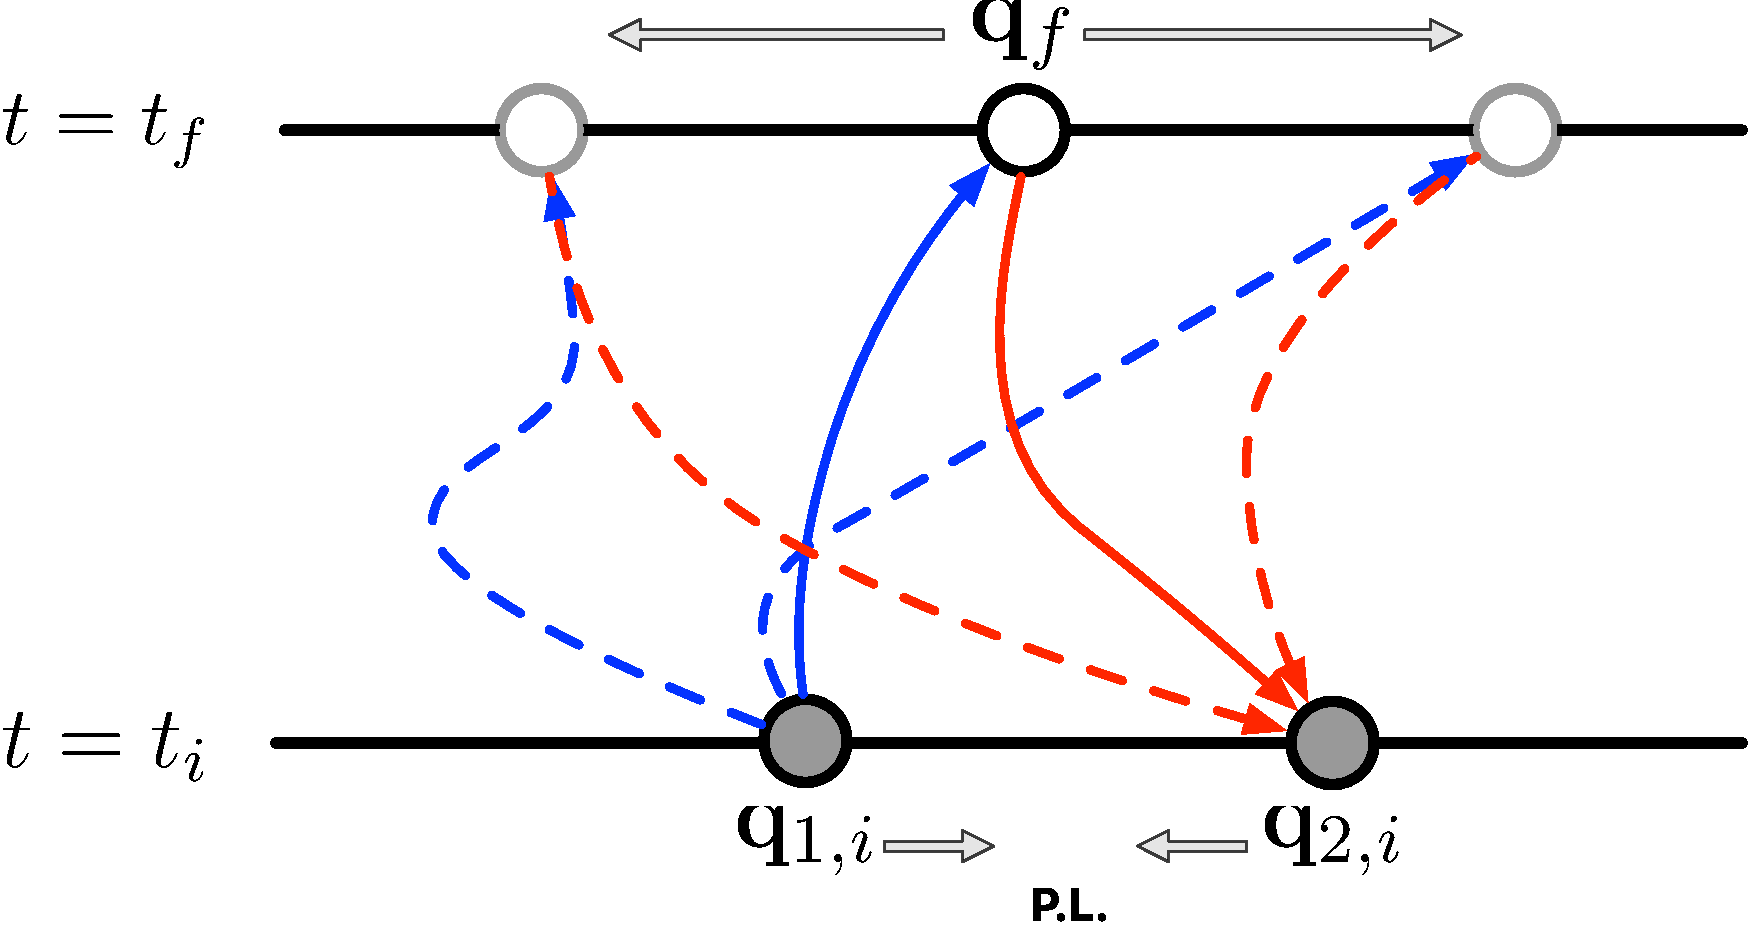
\includegraphics[width=\columnwidth]{figures/qif-two-paths.pdf}
  \caption{A cartoon based on a similar figure from \cite{galleyClassicalMechanicsNonconservative2013} showing the two virtual paths. We can see that the two paths initiate at their respective initial configurations $\vbq_{i,\set{1,2}}$ at time $t_i$ and are connected by the final configuration $\vbq_f$ at $t_f$. This final configuration is unknown and is allowed to vary within the problem (depicted as two alternative values shown in pale either side), depending on the value of $\vbq_{i,\set{1,2}}$. which are fixed during extremisation (displayed in grey). In this manner the problem's boundary resides purely in the $t = t_i$ plane where physical information is known. As shown the physical limit (P.L.) consists of bringing the two virtual paths together such as $\vbq_{i, 1} = \vbq_{i, 2}$.}
  \label{fig:nc-lagrange-virtual-paths}
\end{figure}

This method was originally developed to account for the fact that while we often employ Hamilton’s principle and the Euler-Lagrange equations it produces as an initial value problem, it is formally a boundary value problem in time. To remedy this difficulty we formally double the degrees of freedom of our system into two new virtual paths $\vb q_{1,2}$, with an adapted non-conservative Lagrangian $\Lambda$ given by,

\begin{equation}
  \label{eq:nc-lag}
  \Lambda = L(\vbq_1, \dot\vbq_1, t) - L(\vbq_1, \dot\vbq_1, t) + K(\vbq_1, \vbq_2, \dot\vbq_1, \dot\vbq_2, t).
\end{equation}

The form of this equation, as well as the visualisation shown in \fref{fig:nc-lagrange-virtual-paths}, shows we can consider this doubling as creating two paths, one forwards in time, the other backwards (and hence negative in \eqref{eq:nc-lag}), with both of these paths contribute with terms as the traditional conservative Lagrangian. There is also an additional term $K$, the non-conservative potential, representing a non-conservative coupling between the two paths (if it could be broken down cleanly into a form of $V(\vbq_1) - V(\vbq_2)$or similar, and thus being conservative, then these could be absorbed into $L$ leaving $K = 0$). In this way the system becomes a boundary value problem as needed, with both paths sharing the $\vbq_f$ point as one of their boundaries.

To solve this system we follow in the same form as before, aiming to extremise a new action defined now in terms of $\Lambda$, however crucially we do so in what is known as the \enquote{physical limit} (P.L), where $\vbq_1 = \vbq_2$. This gives the non-conservative Euler Lagrange equation,

\begin{equation}
	\label{eq:nc-el}
  	\left[\frac{\p \Lambda}{\p q_i} - \frac{\dd}{\dd t}\frac{\p \Lambda}{\p \dot q_i}\right]_{\text{P.L}} = 0
\end{equation}

In practical considerations it is often useful to alter our choice of variables to instead be $\vbq_+ = {(\vbq_1 + \vbq_2)}/{2}$ and $\vbq_- = \vbq_1 - \vbq_2$. This reduced our P.L. condition to simply $\vbq_- \to \vb 0$. Note that only the Euler-Lagrange equation involving differentiating wrt. $\vbq_-$ survives. We can of course also define a corresponding conjugate momenta,

\begin{equation}
  \pi_{\mp, i} = \frac{\p \Lambda}{\p q_{\pm,i}}.
\end{equation}

A corresponding form of Noether's theorem can be shown to hold for these non-conservative systems where the Noether currents evolve in time due to the effect of the non-conservative coupling potential $K$ \cite{galleyPrincipleStationaryNonconservative2014}. There one can also find a more complete explanation of the process described above, along with a rigorous derivation.

\subsection{The \SI}
\label{sec:intro-si}

The \SI{} is an extension of a symplectic integrators to non-conservative Lagrangian mechanics, symplectic integrators being those which preserve the canonical symplectic 2-form of the system $dp \wedge dq$, and thus preserve many desired properties during integration.

Hence, to understand the \SI{} method we first consider the application of a symplectic integrators to a traditional conservative system\footnote{This explanation takes its path from an unpublished paper by Tsang \etall \cite{tsangVariationalSymplecticIntegrators}}. As before consider a system with $N$ degrees of freedom represented by some $\vbq \in \R^N$, governed by some Lagrangian, $L(\vbq, \dot{\vbq}, t) \in \R$.

With this set up we now choose to apply two successive procedures to our extremal path $\vb q(t)$: first piecewise breakdown and then discretisation of the action itself. It is this ordering that differentiates this symplectic method from more traditional integrators such as Runge-Kutta \cite{devriesFirstCourseComputational2011} which solve similar systems by discretising the final equations of motion themselves rather than the action, before equations of motion are formed.

To start we break the trajectory down piecewise into a collection of $M$ sub-paths $\gamma_{n \in [M - 1]}$ where $[A] = \set{0, \dots, A}$, each defined on some portion of the whole timespan $[t_n, t_{n + 1}] \subset [t_i, t_f] \subset \R$ such that they cover it completely with overlaps only at the boundaries of the intervals. These together are such that the there is the correspondence,

\begin{equation}
\label{eq:pw-traj}
	\vb q(t) = \begin{cases}
		\gamma_n(t) &\text{for~} t \in [t_n, t_{n + 1}]
	\end{cases}
\end{equation}

between the total path and sub-paths for all $t \in [t_i, t_f]$. These paths define a collection of points $\vb q_{n \in [M]}$ which are their mutual values at the piecewise break points (which we required to be equal) and the initial and final values for $n = 0$ and $n = M$ respectively.

As each piecewise curve constitutes in and of itself a physically attained trajectory we can state that any path $\vb{q}(t)$ which extremises the action for the whole timespan, must also extremise each piecewise portion, and visa-versa. 

This does not bring us closer to a numerical solution directly but allows us to freely split our integral domain as needed without loss of accuracy, and thus limit the error of our numerical-integration method which will necessarily increase with the number of time-steps or their size.

We now turn to the discretisation method itself. This is done using the Galerkin-Gauss-Lobatto (GGL) quadrature method of order $r \in \N_0$\cite{tsangSLIMPLECTICINTEGRATORSVARIATIONAL2015, farrVariationalIntegratorsGravitational2007} which approximates the integral from $t_n$ to $t_{n + 1}$ using the intermediary points

\begin{equation}
  t^{(i)}_n = t_n + (1 + x_i)\frac{\Delta t}{2}
\end{equation}

% NOTE: Orders defined here

where $i \in [r + 1]$ and $x_i$ are the ordered roots of the the derivative of the $(r + 1)$th Legendre polynomial $P_{r + 1}$ and $\Delta t = t_f - t_i$. For a given choice of $r$ this provides slimpletic maps that are accurate up an order $2r + 2$\cite{tsangSLIMPLECTICINTEGRATORSVARIATIONAL2015}. In turn we also define the $\vbq_n^{(i)} = \vbq(t^{(i)}_n)$ to be the interior points to be the value of each sub-path at each $t^{(i)}_n$. This process can be seen visually in \fref{fig:si-process}.

\begin{figure}[t]
  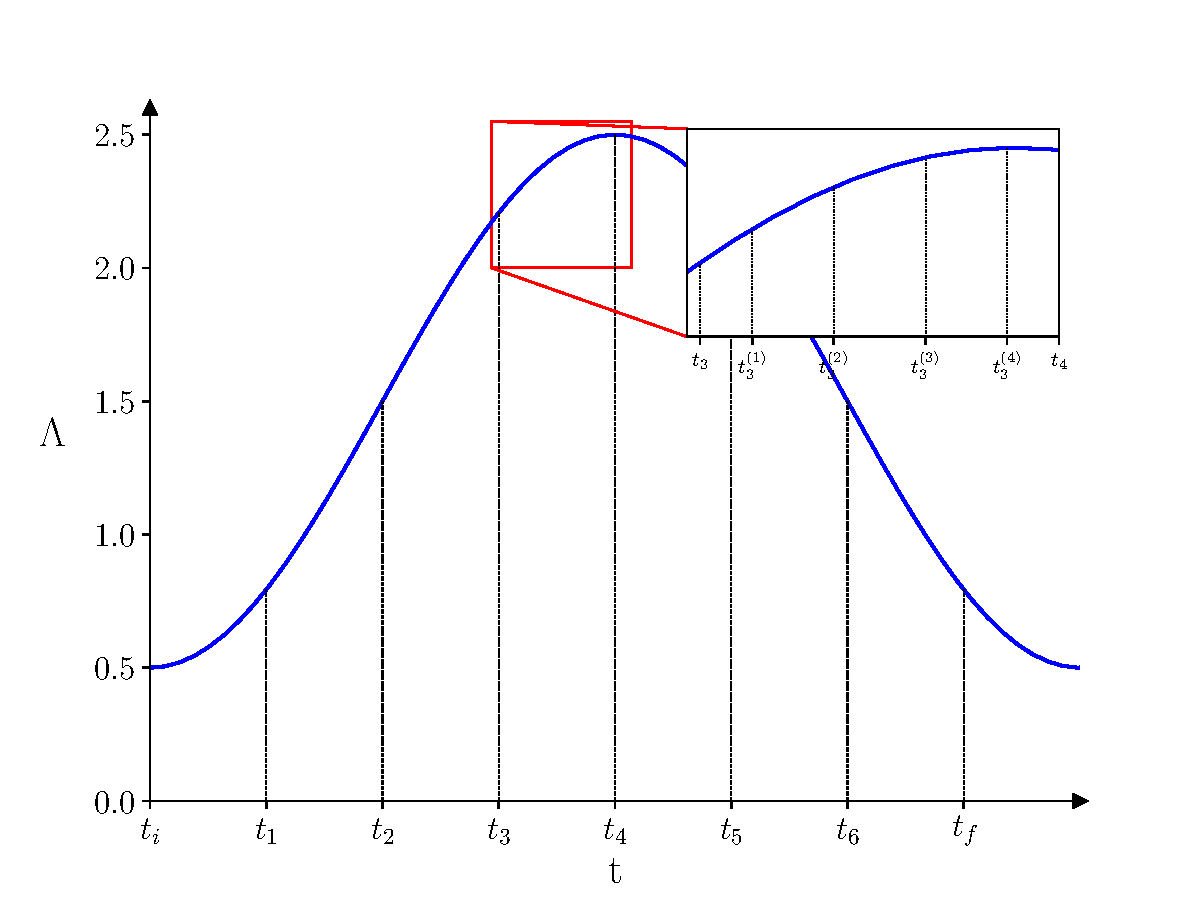
\includegraphics[width=\columnwidth]{figures/si-process.pdf}
  \caption{A depiction of the piecewise breakdown and then discretisation of the action. Each $t_n$ represents shows the action over a subpath $\gamma_n$. In addition we focus on the sub-path spanning $[t_3, t_4]$ showing the interior times $t_{3}^{(i)}$ for $r = 4$.}
  \label{fig:si-process}
\end{figure}

We now approximate the path of the system within this quadrature using the associated cardinal functions for the GGL quadrature, labelled $\phi(t)$, as \(\vb q(t) = \phi(t) + \Or((\Delta t)^{r + 2})\). These provide a suitable approximation for the path derivative $\dot{\vb q}$ by the use the derivative matrix,

\begin{equation}
\label{eq:dij}
  D_{ij} = \begin{cases}
  	\dfrac{(r + 1)(r + 2)}{2\Delta t} &i = j = 0 \\\\
  	-\dfrac{(r + 1)(r + 2)}{2\Delta t} & i = j = r + 1 \\\\
  	0 & i = j \land i \notin \set{0, r + 1} \\\\
  	\dfrac{2P_{r + 1}(x_i)}{P_{r+1}(x_j)(x - x_j)\Delta t} & i\neq j
  \end{cases}
\end{equation}

which provides that,

\begin{equation}
  \dot\phi(t_n^{(i)}) = \sum_{j = 0}^{r + 1} D_{ij}q_n^{(j)}.
\end{equation}

In turn this allows to express the integral as,

\begin{equation}
\label{eq:discr-action-1}
  \int_{t_n}^{t_{n + 1}} L(\vb q, \dot{\vb q}, t) \dd t \approx \sum_{i = 0}^{r + 1} w_i L(q_{n}^{(i)}, \dot\phi_{n}^{(i)}, t_{n}^{(i)})
\end{equation}

where the label the approximate expression $L_d^n$ and where $w_i$ are the quadrature weights given by

\begin{equation}
  w_i = \frac{\Delta t}{(r + 1)(r + 2)(P_{r + 1}(x_i))^2}.
\end{equation}

Equation \eqref{eq:discr-action-1} strung together across the different piecewise sub-trajectories defined in equation \eqref{eq:pw-traj} gives us the total discretised action of the system, shown in Equation \eqref{eq:discr-action-2}, that sets symplectic integrators apart from their more general counterparts,

\begin{align}
\label{eq:ldn}
L_d^n &= \sum_{i = 0}^{r + 1} w_i L(q_{n}^{(i)}, \dot\phi_{n}^{(i)}, t_{n}^{(i)}), \\
\label{eq:discr-action-2}
  S_d &= \sum_{n = 0}^{M} L_d^n.
\end{align}

From here we then extremise this discretised action with respect to the mutual and interior points to obtain the equations of motion of the system as,

\begin{gather}
	\frac{\p L_d^{n-1}}{\p q_n} + \frac{\p L_d^{n}}{\p q_n} = 0 \\
	\label{eq:Ld-interior-eom} \frac{\p L_d^{n}}{\p q^{(i)}_n} = 0.
\end{gather}

This first equation can be simplified further into two equivalent definitions for the discrete momentum \(\pi_n\),

\begin{align}
	\label{eq:pi-n} \pi_n &= -\frac{\p L_d^{n}}{\p q_n} \\
	\label{eq:pi-n+1} \pi_{n + 1} &= \frac{\p L_d^{n}}{\p q_{n + 1}}
\end{align}

and a continuity constraint that they both be equal at these mutual overlap points $\vbq_n$ in the same manner as we required for $\vbq_n$ itself. Together Equations \eqref{eq:Ld-interior-eom}, \eqref{eq:pi-n} can be solved to determine the values of $\vb q^{(i)}_n$, from which Equation \eqref{eq:pi-n+1} provides a form for determining $\pi_{n + 1}$.

This derivation is provided in terms of the traditional conservative Lagrangian $L$ however can be readily adapted to the non-conservative Lagrangian formalism discussed in \sref{sec:intro-nc-actions} by considering instead the non-conservative Euler-Lagrange Equation \eqref{eq:nc-el}, in effect substituting $L$ for the non-conservative Lagrangian $\Lambda$ and $\vb q_n$ for $\vb q_{n, -}$.

Continuing the consideration of Noether currents from prior sections, it can be shown that the continuous symmetries of the conservative action evolve as due to this now discretised $K_d$. It should be noted that GGL discretisation does not preserve time-shift symmetry, and hence energy is non conserved under the operation, however we will show, in line with previous work \cite{tsangSLIMPLECTICINTEGRATORSVARIATIONAL2015}, that the fractional error is generally bounded over the integration.

\subsection{Physics Informed Neural Networks}
\label{sec:intro-pinn}

Physics informed neural networks (PINNs) are neural networks which include physical knowledge in their training processes \cite{raissiPhysicsInformedDeep2017}. Their most common application is to solving PDEs \cite{luDeepXDEDeepLearning2021,mengCompositeNeuralNetwork2020} where we take physically derived knowledge of the system as a prior in training and fit a neural network to solve some PDE incorporating the residuals into the models loss (loss functions will be discussed in more depth in \sref{sec:intro-lf}).

Neural networks more generally are a collection of linear and non-linear components composed together to form complex non-linear functions. At their base level the linear components can be expressed as the simple linear equation \(\vb{y} = W\vb{x} + \vb{b}\) where $W$ is a collection of weights for this component and $\vb{b}$ the biases; and the non-linear components are functions such as sigmoid or $\tanh$ which are included to stop collapse to linearity for the whole composition. These weights, biases, and other variables within the model constitute the model's \emph{parameters}.

This composition is useful in that it can be shown that, with sufficient complexity, these forms are dense in the space of Borel measurable functions and hence can take the place of almost any physical function or mathematical procedure \cite{hornikMultilayerFeedforwardNetworks1989}.

\subsection{Loss functions}
\label{sec:intro-lf}

Loss functions are the primary leaning method of neural networks and in PINNs act as the place where physics steps in to connect our computational model to reality. Loss functions work by attempting to minimise an arbitrary loss value computed from the parameters and a large dataset of known inputs and outputs for the model.

A loss function traditionally takes the form, $\mathrm{loss} = f(y_{\text{true}}, y_{\text{pred}})$ where $f$ is some chosen function and $y_{\text{pred}}$ and $y_{\text{true}}$ are both real vectors in the output space of the model, representing the known models output and the known true output respectively.

Loss functions in PINNs are often comprised of two components. First there is the prediction or physical loss which may for example be made up of the residuals of the model under PDE, boundary, and initial conditions of the system. Secondly there a regularisation loss term which helps to penalise overfitting to the training data, expressed as \enquote{complexity}, within the model. This might be implemented as an $L^2$  of a vector containing all parameters of the model.

Optimising this loss function can be thought of as a traditional minimisation problem, with common choices of the method being Stochastic gradient descent and Adam\cite{kingmaAdamMethodStochastic2017}. These impose various requirements on the loss function, for example generally that it is differentiable\footnote{Although methods exist for non-differentiable functions \cite{daubechiesIterativeThresholdingAlgorithm2003}.} and benefits from other properties such as higher-order differentiability, Lipschitz continuity, and convexity\cite{sraOptimizationMachineLearning2012}. The rate at which these methods apply gradient based updates is determined a provided learning rate, which will often be varied through training to quickly move towards minima during the initial stages, then tuned down to avoid \enquote{jumping} over the minima as we close in on the optimal solution.

\subsection{Lagrangian Embeddings}

Dealing computationally with non-conservative Lagrangians $\Lambda$, for example as an output of a PINN, requires defining some mapping from a collection of real 	numbers, to a form of $\Lambda(\vbq, \dot\vbq, t)$. This can be thought of as a function,

\begin{equation}
  E: \R^n \to \mathbb{L}
\end{equation}

where $E$ is a chosen embedding function and $\mathbb{L}$ is a subset of the overall function space of possible $\Lambda$ values. The choice of embedding necessarily restricts and dictates the systems which the system can deal with thus its choice is crucial in the design of any system. Discussions of different embeddings used in this paper can be found in \sref{sec:eg-sys}. An embedding can either be chosen to represent a system specifically by its physical parameters, or by some arbitrary function approximation scheme such as Fourier series or Taylor expansions.

It should be noted that these embeddings often will not have a unique correspondence with physical Lagrangians, ie the map is not injective up to physical behaviour. This has implications for optimisation in creating multiple minima as will be discussed.

\subsection{Automatic-Differentiation, XLA, and Google's JAX}
\label{sec:intro-autodiff}

Automatic-differentiation is the process of computing the differential of \enquote{regular} code, ie. code that is substantially similar to code that one would normally write, with respect to one or more of its arguments. Google's JAX library \cite{jax2018github} contains one implementation of this in Python which works by passing \enquote{tracers} into the Python code which record the actions done to them such that a differential can be calculated.

JAX also incorporates the XLA (Accelerated Linear Algebra) library \cite{openxla-xla} where it uses similar tracing methods to translate a restricted, but large, subset of Python code into a series of low-level eifficent operations which can be executed at speed on the GPU or CPU.

These two technologies together show great promise in the fields of machine learning and simulation techniques as they allow for code that would previously have to be written in low-level languages such as C or C++ to be expressed in Python with significantly reduced overhead at runtime, and easier use by researchers.

\section{Method}
%\subsection{Example Systems}
%\label{sec:eg-sys}
%
%When testing our model we employ a number of example systems to test various features of the integrator, in different physical scenarios. Each of these is also associated with a specific embedding.

%\subsubsection{Damped Forced Harmonic Oscillators}
\subsection{Damped Forced Harmonic Oscillators}
\label{sec:eg-sys}

The main physical system used in the testing, and evaluation, of our model is the damped forced harmonic oscillator. It is one of the simplest non-conservative systems, having a non-conservative Lagrangian given by \cite{galleyPrincipleStationaryNonconservative2014},

\begin{equation}
\label{eq:dho-sys-embedding}
\begin{aligned}
  \Lambda &= L - K \\
  L &= \frac12 m\dot\vbq^2 - \frac12 m\dot\vbq -  \\
  K &= - \lambda\vbq_- \cdot \dot \vbq_+ + \vbq_- \cdot \vb{F}(t)
\end{aligned}
\end{equation}

for a system with mass $m$, spring constant $k$, damping constant $\lambda$ and time dependent force $\vb{F}(t)$. This corresponds with the standard equation of motion,

\begin{equation}
  m \ddot{\vb x} + \lambda \ddot{\vb x} + k \vb x = \vb F(t).
\end{equation}

\subsection{Improvements to the \SI{} and their Physical Applications}

Initially, the existing \texttt{slimplectic} codebase from Tsang \etall \cite{originalCode}, which we will refer to as the \orgimpl{}, was rewritten using the JAX framework, known as the \updimpl{}. We chose two key metrics, run-time duration and accuracy, to judge our model against the \orgimpl{} and Runge-Kutta to various orders.

First, to ensure that we maintained the error bounds expected for our model (as per \sref{sec:intro-si}) we compared the fractional energy and momentum error for Runge-Kutta, the \orgimpl{}, and the \updimpl{} across the time evolution of a physical system.

Next, we create two test cases to measure the performance of the integrator and its consequences on experimental capability. These were,

\begin{enumerate}
	\item Modelling systems for different timespans varying the number of iterations performed by the integrator.
	\item Modelling the same system across different orders of integration $r$ to determine how the order of our method affects the performance.
\end{enumerate}

These are designed to test the scaling behaviours of our model to provide insight into its applicability to larger systems.

\subsection{Applications to Loss Functions and Optimisation}

Taking this \updimpl{} we then explore its different uses as a loss function for physical systems, in combination with different embedding functions.

While these are distinct components of the model, they are heavily linked, as ideally, we would define the physical components of our loss function primarily in terms of the trajectories, rather than the values of the embedding vector for the non-conservative Lagrangian itself.
Hence the embedding function and Slimplectic integrator must be chained together, before the physical loss component, to provide it with the trajectories.

We consider a number of choices for these two functions, comparing their behaviour near known minima, and looking for convexity and smoothness. In addition, we also empirically test the suitability of these spaces for optimisation, by directly performing gradient descent to the loss function + embedding composition attempting to converge to a known embedding.

\subsection{Loss Function in the Training of PINNs}

Finally, we employ a loss and embedding function combination to a, simplified, stand-in neural network, observing the correctness of the outputs.

This model was based on the long short-term memory (LSTM) layer \cite{hochreiterLongShortTermMemory1997} which is frequently used in time-series analysis, and thus chosen as a suitable basis for our model. This involves generating large datasets of different physical systems within the domain of the chosen embedding as will be discussed.

\section{Results and Specific Discussion}

\subsection{Improvements to the Slimplectic Integrator and their Physical Applications}
\label{sec:results-si}

\begin{figure}[t]
  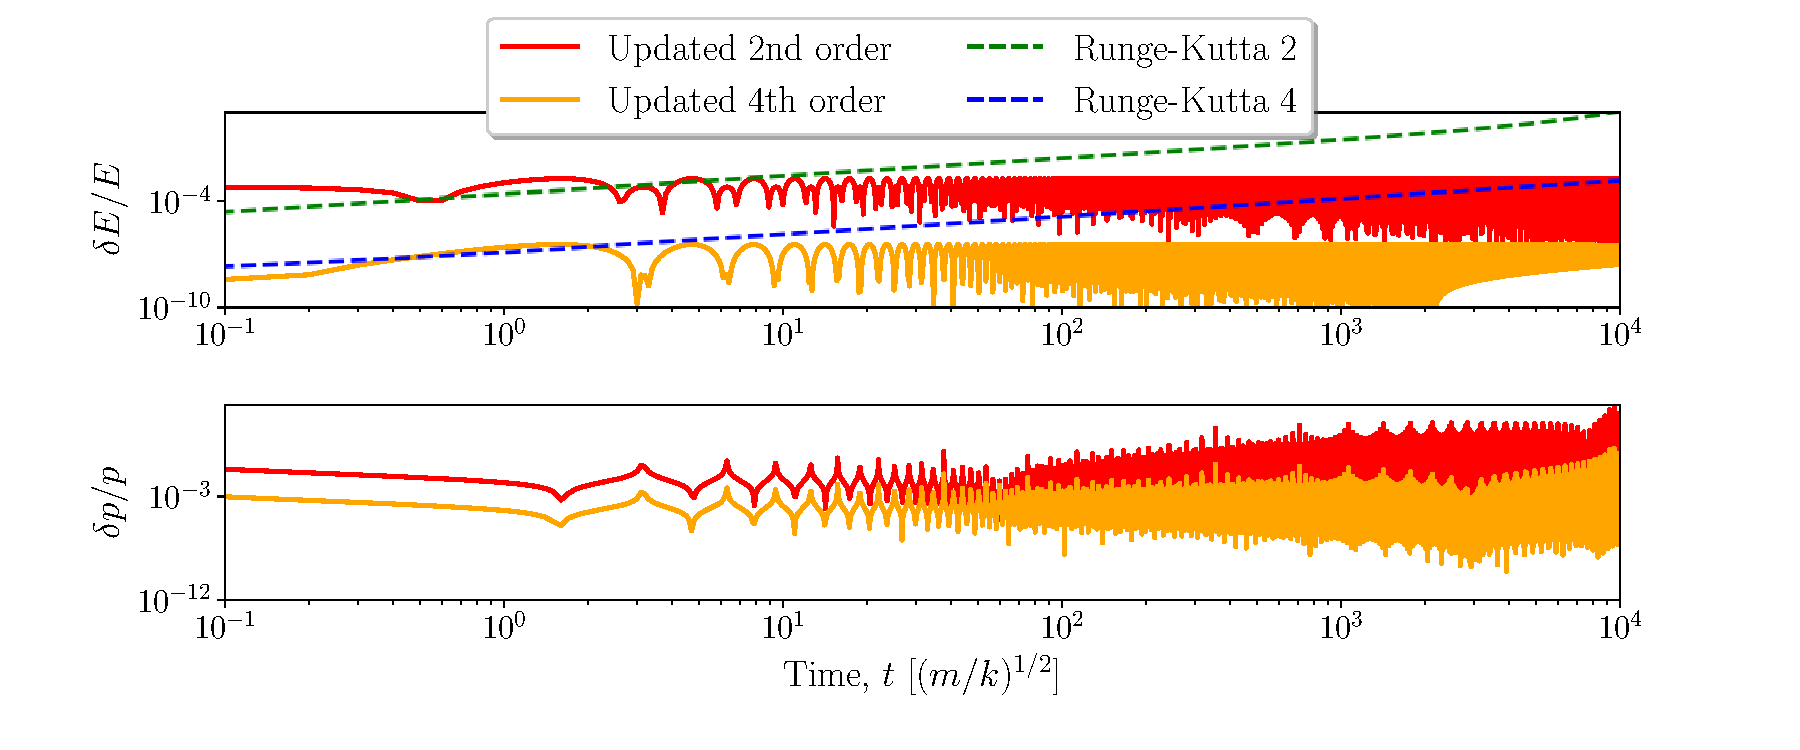
\includegraphics[width=\columnwidth]{figures/dho_energy_momenta_fractional_err.pdf}
  \caption{A comparison of the error in the energy, top, and momenta, bottom, as a fraction of the known analytic solution of the system, of the \updimpl{} simulating a damped harmonic oscillator. One can clearly observe that the fractional energy error is bounded and displays the oscillating behaviour that we expect from previous work, whereas the momenta error does not display such behaviour. This plot is based off its equivalent in the original paper \cite[Figure 2, bottom]{tsangSLIMPLECTICINTEGRATORSVARIATIONAL2015}.}
\label{fig:dho_energy_bounds}
\end{figure}

As discussed we first verify that the \updimpl{} retains required fractional error bounds of the formal method. This can be seen in \fref{fig:dho_energy_bounds} where the fractional error of the \updimpl{} with respect to that of the true analytic solution is compared directly against that of Runge-Kutta order 2 and 4. We clearly observe that the fractional energy error remains bounded across the timeframe of iteration.
This successfully replicated the behaviour of the original implementation to an absolute root mean squared residual over the simulation duration of $\Delta = 1.42 \times 10^{-13}$ and $\Delta = 4.50 \times 10^{-12}$ for $r = 2$ and $r = 4$ respectively.
This is not the case for the fractional momenta error however as fixed-time-step variational methods such as those implemented cannot be both slimplectic-momentum and momentum-energy preserving \cite{zhongLiePoissonHamiltonJacobiTheory1988}.

\begin{figure}[t]
  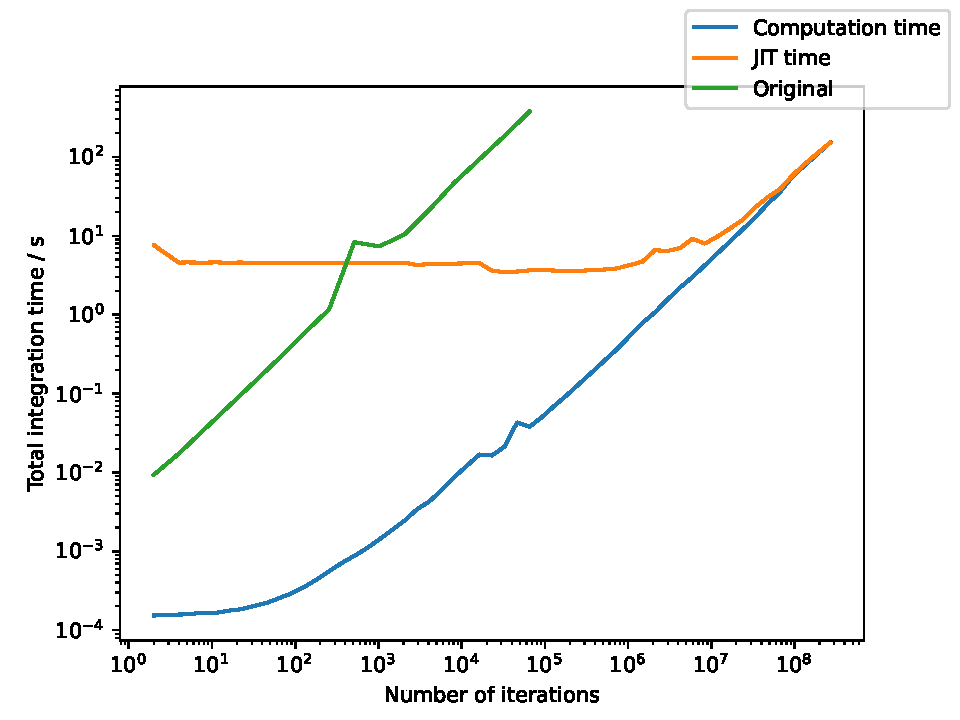
\includegraphics[width=\columnwidth]{figures/dho_n_runtime.pdf}
  \caption{A comparison of running a damped harmonic oscillator system for various numbers of iterations, with $r = 2, \Delta t = 0.1$. The \updimpl{} runtime is split into two components where \ensquote{JIT time} represents the one time fixed cost of compiling the function (see \sref{sec:intro-autodiff}) and \enquote{Computation time} represents the actual time spent on computation.
  Each value is the mean of 4 runs, with the \orgimpl{} being cut off early due after $> 20$ minutes runtime for the next sample.}
  \label{fig:dho-n-runtime}
\end{figure}

\begin{figure}[t]
  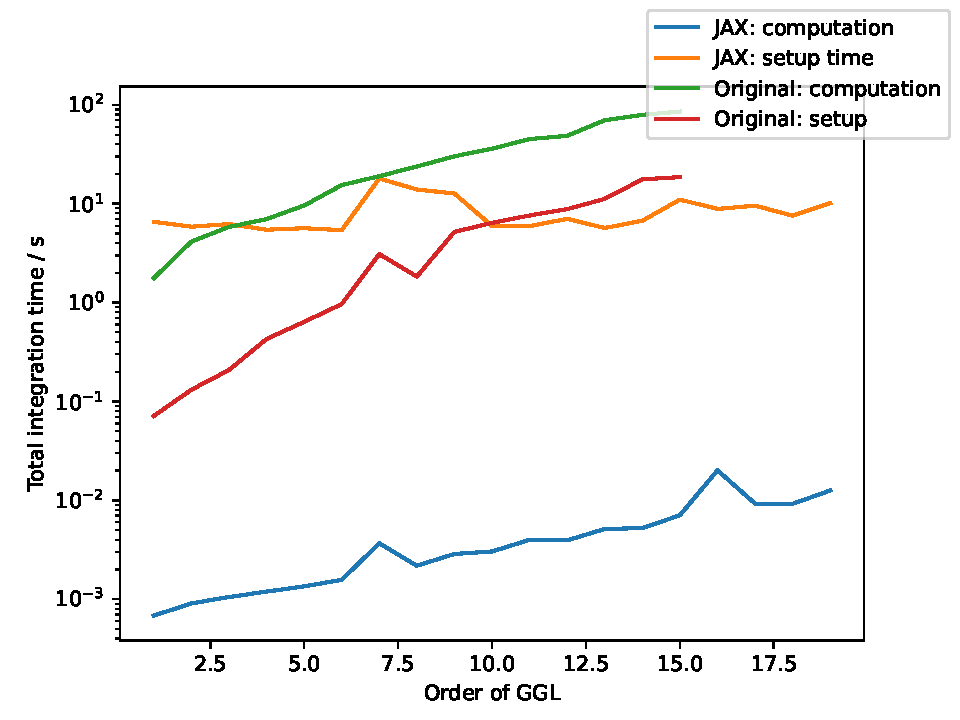
\includegraphics[width=\columnwidth]{figures/dho_r_runtime.pdf}
  \caption{A comparison of running a damped harmonic oscillator system for various values of $r$, the order of the GGL quadrature, with $\Niter = 500, \Delta t = 0.1$. Each result being the mean of 4 independent runs.
	For both implementations we split the overall time into setup and computation as changing the method order requires re-discretising the Lagrangian and thus non-trivial work under both implementations.}
  \label{fig:dho-r-runtime}
\end{figure}

Next we explored the time complexity of the system in terms of the iteration count, $N_{\text{iter}}$, and GGL quadrature order, $r$. These are important to physical applications as they determine the limits of iteration accuracy when iterating over large timescales -- with error scaling as $(\Delta t)^{2r + 2}$ and total timeframe being $N_{\text{iter}} \Delta t$.

Focusing first on the time complexity in $N_{\text{iter}}$ as shown in \fref{fig:dho-n-runtime}, we note that that the computation time of the \updimpl{} is much lower than that of the \orgimpl{}, with the \updimpl{} growing as $\Or((\Niter)^a)$ where $a = 1.0140 \pm 0.0042$. 
In addition we note that the fixed cost JIT compilation remains roughly constant until $10^7$ iterations after which it begins to grow linearly.

This pattern is seen also in \fref{fig:dho-r-runtime} when investigating the time-complexity in the order of the method. Again the JIT time remains roughly constant across the domain tested, and though it starts out initially higher than than the \orgimpl{}'s setup costs, the \orgimpl{}'s computation time quickly swamps this fixed cost.
Similar to the behaviour in $\Niter$, the computation time for the \updimpl{} is also linear $r$ , remaining insignificant in the overall runtime. This is in comparison with the \orgimpl{} where the setup time grows as $\Or(r^n)$ with $n = {2.31 \pm 0.15}$ and the computation time as $\Or(r^m)$ with $m={1.490 \pm 0.070}$.

It should be noted that while increasing the order of the method will increase the precision, at higher orders we start encountering limitations with the fixed precision \texttt{float64} type used for calculation in the \updimpl{} compared the the arbitrary precision numerics employed in the \orgimpl{}.
Still however this represents an overall improvement in accuracy in physically meaningful simulations as the required precision could be more readily attained by decreasing $\Delta t$ rather than increasing $r$, avoiding the blowup of runtime observed in the \orgimpl{}, or the degradation of precision at high $r$ in the \updimpl{}. This is discussed further in \sref{sec:results-si}


\subsection{Loss Functions and Optimisation}
\label{sec:res-lf}

\todo{this first sentence needs re-wording}
Moving now onto the loss function and choice of Lagrangian embedding function. We explored a number of loss functions through a combination of gradient-descent and visual inspection.

A wide number of loss functions were tested, however focusing on those surrounding systems of harmonic oscillators, we settled on DHO system specific embedding shown in equation \eqref{eq:dho-sys-embedding}, labelled DHO 3.
As well an adaption where an additional embedding parameter $\alpha$ was introduced as pre-factor on the entire non-conservative Lagrangian $\Lambda$, labelled DHO 4. 
These were paired with a number of simple loss functions, \tref{table:loss-fns}, drawing from physical knowledge and existing convention for neural network loss functions.

First we perform a visual inspection of the \enquote{Simple RMS} loss function at various scales with both embedding functions, as seen in \fref{fig:loss-function-behaviour}. Here we observe mild non-convexity around the minima, as impulse like behaviour around the highly non-physical $m = 0$ point.

To test how this mild non-convexity translates into optimisation performance we subject a number of combinations to empirical optimisation tests where we attempt to attain a known true embedding from a number of random initial embedding values. \Tref{table:optimisation-results} (see caption for details) shows that that the addition of the global pre-factor $\alpha$ substantially increases the probability of successful convergence.  In addition we see that both the $\vbq$ and $\pi$ values are important in the fitting process from the complete lack of convergence when only $\pi$ is included, and that their relative weight seems to be of little importance at this stage.

This is promising as, while optimisation directly in the embedding space is a strictly simpler problem than with respect to the parameters of an associated neural network, it suggests that this mild non-convexity observed during visual inspect is an obstacle we can overcome.

\begin{figure*}[t]
  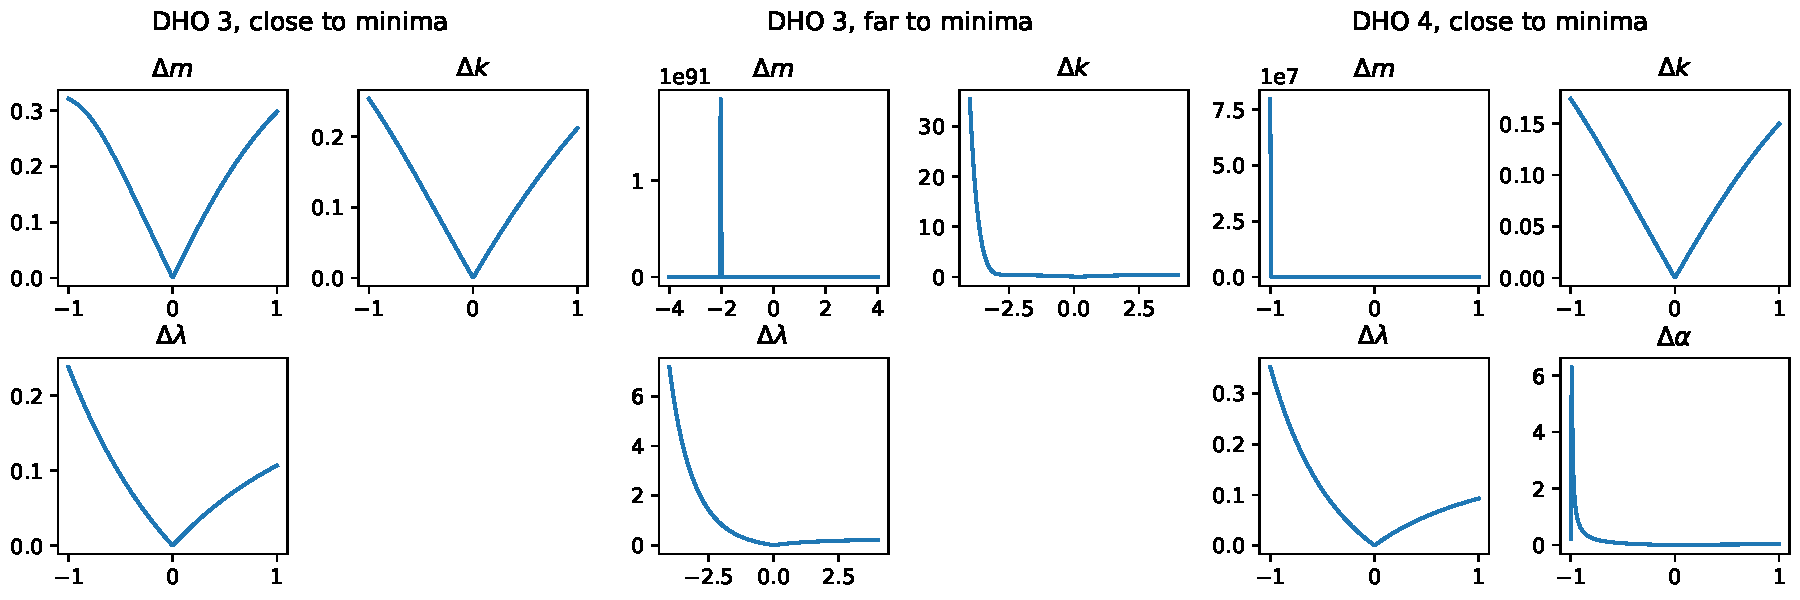
\includegraphics[width=\textwidth]{figures/loss-function-behaviour.pdf}
  \caption{The local behaviour of an equally weighted $\vbq$ and $\pi$ RMS loss function, when viewed as a function of variation in each of the embedding variables independently, with others kept fixed. We observe roughly correct behaviour in all variables bar mass $m$ and subsequently $\alpha$ for the DHO 4 embedding where $\alpha$ acts as a pre-factor for the whole non-conservative Lagrangian $\Lambda$. This behaviour is to be expected as system without mass is non-physical and explodes to infinity.}
  \label{fig:loss-function-behaviour}
\end{figure*}

\begin{table}
\label{table:loss-fns}
\centering
\caption{A list of loss functions. Key: RMS = Root Mean Squared, a standard loss function in machine learning.%; inv-exp t.w. = inverse exponential time weighting.
}
\begin{tabular}{c|p{0.5\linewidth}}
  Name & Description \\
  \hline
  Simple RMS & Sum of RMS for $\vbq$ and $\pi$ in equal weighting. \\
  RMS-$(a, b)$ & Sum of $a$ times the RMS for $\vbq$ and $b$ times the RMS for $\pi$. \\
%  RMS inv-exp t.w. & Weighting the contribution from each time-step by $e^{-t}$  \\
\end{tabular}
\end{table}

\begin{table}
\label{table:optimisation-results}
\centering
\caption{Results of optimising the chosen loss function from \tref{table:loss-fns} for $200$ initially random embeddings (distributed uniformly in $[0, 10]^n$) in the input space of the chosen embedding function, where convergence is defined as being within $\epsilon = 0.05$ of the true embedding at the end of a maximum of $250$ iterations of the optimiser. Note that for DHO 4 an additional normalisation step of dividing by $\alpha$ was applied to remove the redundancy introduced by the pre-factor in when determining if convergence had been achieved. The true embedding that was optimised towards, in DHO 3 form, was $(m = 2, k = 3, \lambda = 1)$ and systems were compared with $\Niter = 50, r = 2, \Delta t = 0.1, q_0 = 0, \pi_0 = 1$.}
\begin{tabular}{l|l|c}
  Loss function & Embedding & Convergence $\%$ \\
  \hline
  Simple RMS & DHO 3 & $33.5\%$ \\
  Simple RMS & DHO 4 & $97.5\%$ \\
  RMS-$(2, 1)$ & DHO 4 & $98\%$ \\
  RMS-$(0, 1)$ & DHO 4 & $0\%$ \\
%  RMS inv-exp t.w. & DHO 3 &
\end{tabular}
\end{table}


\subsection{PINNs and Approximating Damped Harmonic Oscillators}

Finally, we applied these techniques to a PINN. For our initial explorations in this space, we focused on fitting to systems of damped harmonic oscillators as has been the through line of the work thus far. We chose the 3-parameter DHO embedding over the 4-parameter embedding with a pre-factor as while DHO 4 was more effective when subject to direct gradient descent, we were concerned that the additional redundant embedding parameter would make learning the systems more complex and error-prone.

The dataset used in training ($N \approx 5 \times 10^5$) was a mixed selection. Primarily it was comprised of uniformly distributed embeddings within the subset of the physical region of the embedding space (positive embedding values). In addition a fraction, approximately $5 \%$ for both, of the spring and damping constants were set to zero to ensure that the model was exposed to non-damped simple harmonic motion and kinetic energy only systems.

For PINN training, accounting for the increased complexity of the optimisation problem now being with respect to the parameters of the model, we made two alterations to our loss functions. First, we added a strong weight against non-physical negative embedding values in our loss function, taking the form of,

\begin{equation}
  f(e_i) = \begin{cases}
  	0 & e_i \ge \delta \\
  	\exp{-\gamma e_i} & e_i < \delta 
  \end{cases}
\end{equation}

where $\delta = −0.1$ is a tolerance to allow for zero to be a non-penalised output and $\gamma \approx 10$ is the strength of the penalisation. This was done as the non-physical behaviour of negative embedding values is less visible when considering the larger whole model optimisation problem.
In addition, we also experimented with capping the values of the loss at large values to mitigate overflows when dealing with particularly bad fits, such as the initially random initialised weights before any training had commenced. Both of these alterations notably improved training stability and decreased the probability of floating-point related errors.

Model training was done in batches and was prone to explosion possibly due to the non-convexity in some regions as discussed in \sref{sec:res-lf}. Overall it was found that training could be made more stable by increasing batch sizes to $512$ from $32$, and manually tweaking learning rates and loss weightings (for example between the $\vb q$ and $\pi$ RMS terms where more progress was made with weighting towards $\vbq$ error to counteract observed larger tendency for error in this term) as training progressed.

Other loss functions, such as RMS in $\pi$ only (RMS-(0, 1) in \tref{table:optimisation-results}), were once again investigated. This initially looked promising, producing good losses on the order of $10^{-4}$, however on further inspection it was found that these resulted from a finding a false minima of $m \approx k \approx \lambda$, highlighting the complexity of the embedding space in representing physical systems. This also underlined the utility of the previous direct embedding space optimisation done prior in informing us about the behaviour of the loss function itself.

By the training's conclusion we obtained an absolute RMS error of $\pm 5 \times 10^{-2}$ in $\vbq$ and $\pm 1 \times 10 ^{-1}$ in $\pi$. This model was able to predict systems with some accuracy, clearly able to fit to certain features as shown in \fref{fig:model-prediction}.

\begin{figure}[t]
  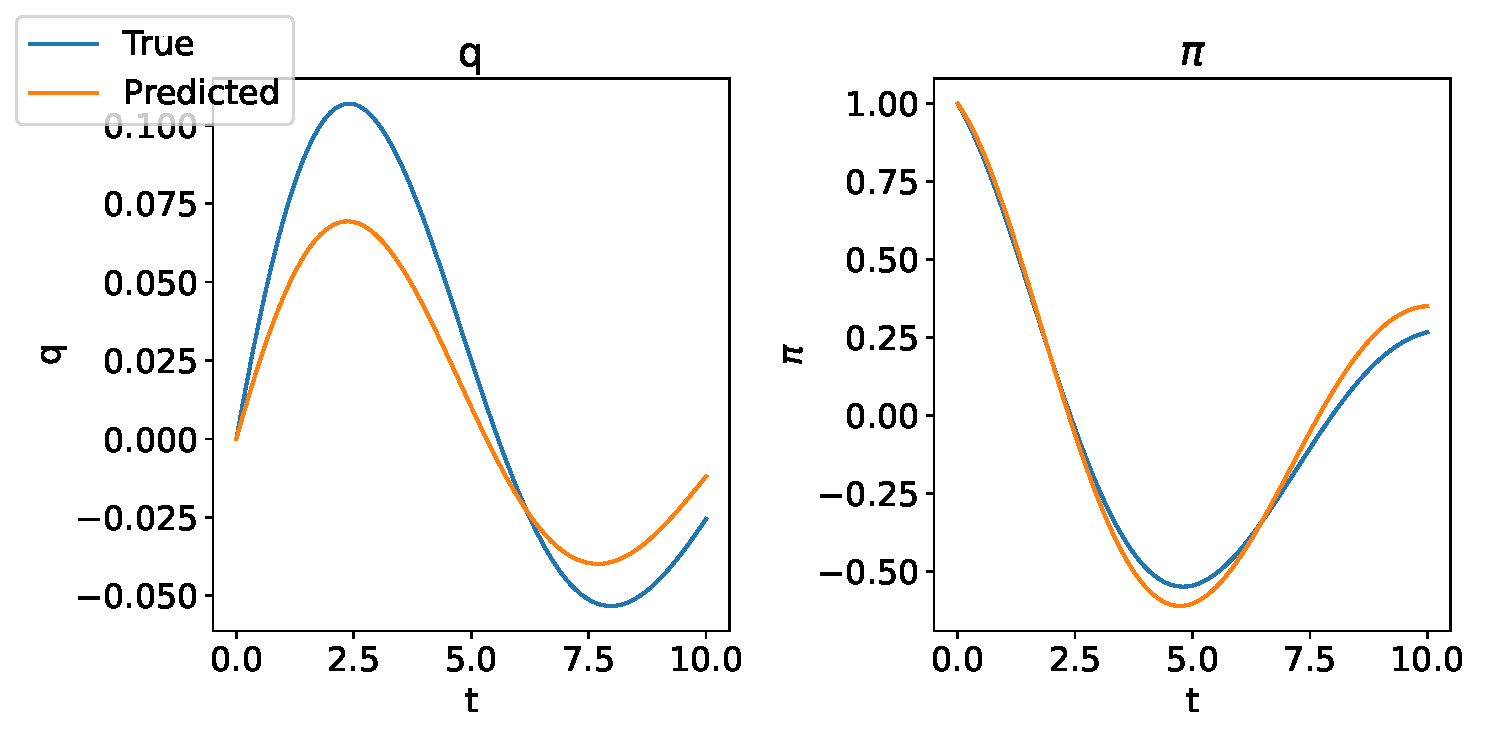
\includegraphics[width=\columnwidth]{figures/model-predictions.pdf}
  \caption{A comparison of the behaviour of a Lagrangian embedding predicted by a PINN. True embedding, $(m = 6, k = 2, \lambda = 3)$, predicted embedding, $(m = 9.401553,  k = 3.3729377, \lambda = 3.9162085)$.}
  \label{fig:model-prediction}
\end{figure}



\section{Discussion}

\subsection{\SI{}}

We have presented a number of results on the performance characteristics of the \updimpl{} of the \SI{} method when applied to physical problems which warrant additional discussion to place them in context.

Starting with the effect of changing the method order $r$, as presented in \fref{fig:dho-r-runtime}.
Roughly constant-time behaviour is observed and is expected to continue for higher values of $r$ as this reflects very little change in the size of the underlying calculation (due to data-size and calculation cost) involved in the integration process.
This, coupled with the ability to split long integration runs (high $\Niter$ values) into multiple successive runs, means, that with careful management of errors (especially with regards to round-off build up due to fixed precision floats), we should be able limit to the degradation to linear performance observed in \fref{fig:sho-n-runtime} for $\Niter > 10^7$.
From this $\Niter$ value the method's internal arrays become greater than 1Gb in size possibly hitting JAX de-optimisation.

It is important to note however, that in the high order domain $r \gtrsim 40$ the computation of the derivative matrix, given in Equation \eqref{eq:dij}, begins to fail as we encounter issues with the \texttt{float64} floating point precision used in JAX calculations. Unfortunately, this is unavoidable as it is the maximum precision offered by JAX. Nonetheless, this limitation can be mitigated, whilst retaining the desired error characteristics, by employing alternative strategies, such as reducing the time step or using a higher-order method with a lower value.

Overall, however this approach is made more fruitful by noting that we can avoid the fixed cost entirely if we reuse the same of form non-conservative Lagrangian. This allows us to vary not only initial conditions, for example exploring the same system in different circumstances or restarting after multiple runs, but also sample across a range of physical parameters (such as those parameterising the DHO 3 embedding as defined in Equation \eqref{eq:dho-sys-embedding}). In particular this scaling without fixed costs applies effectively to systems composed of many repeated sub-systems such as field theory or molecular dynamics simulations \cite{tuckermanUnderstandingModernMolecular2000b}.

As shown in \fref{fig:dho-n-runtime}, we observe a transient increase in runtime over the range $r \in [7, 9]$. This phenomenon is repeatable and its origin is uncertain. However, informed by the size of the quadrature array being $r + 2$, we suspect that this behaviour is due to optimisation cliffs in the JAX internal code as we transition between two internal implementations optimised for small vs large array sizes. Finally, it is important to consider that for less trivial systems, where evaluating the Lagrangian may bring its own performance considerations, the method may require further analysis and optimisation.

Looking forwards, we noted that the use of fixed time steps in the method limits our ability to maintain energy and momentum fractional error bounds. Moving to an adaptive time step approach would be a promising avenue for improvement in future work.

\subsection{PINN, Current and Future}

The trained neural network represents a promising first step in predicting non-conservative Lagrangians from observational data successfully capturing the general characteristics of the data.
During our experiments, we frequently observed predicted embeddings with values of roughly correct proportion, but off by a constant factor. This suggests that the 4 parameter embedding or other normalisation method may have been useful as the model was unable to move past this local minima in phase space, representing a sufficiently similar physical system. \todo{say something about this}
This poses questions on the handling of degeneracy in our Lagrangian space where multiple Lagrangians can result in the same physical system, especially within the image of any chosen embedding function, as this degeneracy will present issues when optimising within the space.

Furthermore, we noted that the model was substantially more accurate with comparatively high masses. We theorise that this may be due to difficulties in fitting larger values of $\vbq$, possibly indicating the need for a larger and more varied dataset. It is important to acknowledge that this was a simplified test network, and we anticipate that future work will achieve improvements by utilising a larger parameter count and datasets.

To enhance the model's performance, incorporating physically known a priori information into the loss function may be beneficial. For example, a stricter restriction on non-negativity for the DHO 3 parameters could be implemented by first taking the absolute value of the outputs as inputs to the Slimpletic Integrator. This would have the effect of cleanly solving the problem of non-physical embedding values, at the cost of introducing additional degeneracy into our space possible confusing the model.

It should be noted however that this approach, and others like it, present a trade-off between specialising our embedding functions and loss functions towards a particular physical systems where we have more physical knowledge and create models which are more widely applicable (for example through the use of Taylor series embedding functions).
Identifying physical laws that can be enforced in the Lagrangian would be a fruitful avenue for future research.

Following this theme, a suitably trained neural network could be constructed using this method to identify symmetries in observational data or recognise patterns it has previously been exposed to in new observational data. This suggests potential applications in domains such as astrophysics, where there is a large availability of data to train a model, but also difficulties in obtaining a complete dataset for any one experiment.

\section{Conclusion}

In this paper we have put forward a more optimal implementation of the Slimpletic Integrator, which is capable of scaling to large scale physical simulations while preserving bounded fractional error in the energy. We have shown this implementation has applications in the construction of a loss function for physics informed neural networks, and presented a simple model which shows that this approach has promise for identifying non-conservative Lagrangians from observational data. More work is required to explore better encodings of physical invariants in the loss function and model structure.


\ack

\begin{enumerate}
	\item Tsang, resources
	\item Do we need to reference the Royal Society?
	\item Mathilda, Dunkun
\end{enumerate}

\section*{References}
\bibliographystyle{iopart-num}
\bibliography{references,static}

\end{document}
